\section{Virtual Reality}\label{sec:virtual-reality}

Virtual Reality is a term used to describe interactive, immersive, and realistic, 3D computer simulated environments.
The main factor distinguishing this technology from other media is the ability to consistently generate compelling
feelings of presence, immersing the user fully in a synthetic environment that allows natural interaction and
participation as if they were in the real world~\cite{Davis2014}.
Such environments and corresponding technology were described as early as 1965 by Ivan E. Sutherland, who also created
what is widely believed to be the first head-mounted display~\cite{Sutherland1968}.
Since this first prototype, there has been a continuous effort and development over the last 50 years to improve the
tools and technologies for interacting with, and inspecting virtual environments.
Recently, these developments achieved further breakthroughs and increased public interest with the emergence of
easily accessible position tracking technology in the entertainment sector, such as Nintendo's Wii, and Microsoft's
Xbox Kinect.

\begin{figure}[h]
    \centering
    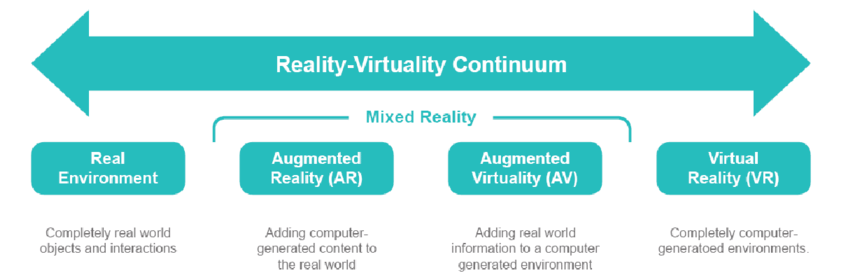
\includegraphics[width=\textwidth]{content/2_1_virtual_reality/img/reality-virtuality-continuum[Spivak2015]}
    \caption{Reality-virtuality spectrum adapted by~\cite{Spivak2015} from~\cite{Milgram1994}.}
    \label{fig:environment-spectrum}
\end{figure}

Milgram and Kishino~\cite{Milgram1994} proposed a taxonomy to classify virtual reality and adjacent technologies that
emerged.
The spectrum ranges from real environments, over mixed reality, where either computer generated content is inserted
into the real world (Augmented Reality, AR), or real world information and objects are used to enhance a computer
generated world (Augmented Virtuality, AV), all the way to Virtual Reality (VR) at the far end of the spectrum
(Figure~\ref{fig:environment-spectrum}).
The devices used for virtual reality can vary similarly in size and immersion.
The most prevalent technologies for mixed and virtual environments are the Computer Aided Virtual Environments (CAVEs),
where multiple images are projected in a room, that are viewed through stereoscopic glasses, and head-mounted
displays (HMDs), where stereoscopic images are produced by displays mounted in a headset.
The latter has gained increasing popularity in main stream media with the Kickstarter, and release of the Oculus Rift,
and the subsequent products released by Oculus, HTC VIVE, and Valve.

The key technology for virtual and mixed reality devices is stereoscopic display, where the left and right eye are
provided with offset views, imitating the real world view on a virtual scene, and thus providing the user with a
realistic depth perception.
There are different methods to provide stereoscopic images to the user:
\begin{itemize}
    \item Passive filters, where polarizing filters ensure each eye only sees the intended image, while both views
    are displayed in an interlaced stream.
    \item Active filters, where "shutter-glasses" turn the lenses opaque using a timing signal to ensure each eye
    only sees the intended image in an interlaced video stream.
    \item Independent displays, where each eye has a dedicated display showing the offset view.
\end{itemize}

With these advances and VR HMDs becoming more consumer-friendly and affordable, virtual and mixed reality present a
new style of intuitive human-computer interfaces with the primary goal to increase communication bandwidth between
human and computer through immersion in a synthetic environment~\cite{Davis2014}.
Examples of this are the increased use of VR to train individuals in tasks, that are too difficult, dangerous, or
expensive otherwise.
Additionally, VR has been successfully used in medical treatments to treat anxiety disorders, like phobias and
post-traumatic stress syndrome (PTSD)~\cite{Clifton2020}.
Lastly, VR technology is used in different domains for visualisation and intuitive interfaces, like healthcare,
construction, architecture, and research.
